%%%%%%%%%%%%%%%%%%%%%%%%%%%%%%%%%%%%%%%%%
% University Assignment Title Page
% LaTeX Template
% Version 1.0 (27/12/12)
%
% This template has been downloaded from:
% http://www.LaTeXTemplates.com
%
% Original author:
% WikiBooks (http://en.wikibooks.org/wiki/LaTeX/Title_Creation)
%
% License:
% CC BY-NC-SA 3.0 (http://creativecommons.org/licenses/by-nc-sa/3.0/)
%
% Instructions for using this template:
% This title page is capable of being compiled as is. This is not useful for
% including it in another document. To do this, you have two options:
%
% 1) Copy/paste everything between \begin{document} and \end{document}
% starting at \begin{titlepage} and paste this into another LaTeX file where you
% want your title page.
% OR
% 2) Remove everything outside the \begin{titlepage} and \end{titlepage} and
% move this file to the same directory as the LaTeX file you wish to add it to.
% Then add \input{./title_page_1.tex} to your LaTeX file where you want your
% title page.
%
%%%%%%%%%%%%%%%%%%%%%%%%%%%%%%%%%%%%%%%%%
%\title{Title page with logo}
%----------------------------------------------------------------------------------------
% PACKAGES AND OTHER DOCUMENT CONFIGURATIONS
%----------------------------------------------------------------------------------------

\documentclass[12pt]{article}
\usepackage[english]{babel}
\usepackage[utf8x]{inputenc}
\usepackage{amsmath}
\usepackage{graphicx}
\usepackage[colorinlistoftodos]{todonotes}
\usepackage[none]{hyphenat}
\usepackage{hyperref}
\usepackage{caption}

\setlength{\parindent}{0pt}
\frenchspacing

\newcommand{\quotes}[1]{``#1''}
\newcommand{\comment}[1]{}

\begin{document}

\begin{titlepage}

\newcommand{\HRule}{\rule{\linewidth}{0.5mm}} % Defines a new command for the horizontal lines, change thickness here

\center % Center everything on the page

%----------------------------------------------------------------------------------------
% HEADING SECTIONS
%----------------------------------------------------------------------------------------

\textsc{\LARGE University Of Windsor}\\[1.5cm] % Name of your university/college
\textsc{\Large 60-367}\\[0.5cm] % Major heading such as course name
\textsc{\large Computer Networks}\\[0.5cm] % Minor heading such as course title

%----------------------------------------------------------------------------------------
% TITLE SECTION
%----------------------------------------------------------------------------------------

\HRule \\[0.4cm]
{ \huge \bfseries Botnet Research Paper}\\[0.4cm] % Title of your document
\HRule \\[1.5cm]

%----------------------------------------------------------------------------------------
% AUTHOR SECTION
%----------------------------------------------------------------------------------------

% If you don't want a supervisor, uncomment the two lines below and remove the section above
\Large \emph{Author:}\\
Quinn Perfetto - 104026025\\[3cm] % Your name

%----------------------------------------------------------------------------------------
% DATE SECTION
%----------------------------------------------------------------------------------------

{\large \today}\\[2cm] % Date, change the \today to a set date if you want to be precise

\vfill % Fill the rest of the page with whitespace

\end{titlepage}


\tableofcontents

\pagebreak

\section{Introduction}

A botnet is a private network of computers infected with malicious software which allows them to be controlled by an entity known as the \textbf{Command and Control (C\&C)}.
The infected computers, referred to as \textbf{zombies}, are generally unaware that they are members of the botnet.
Botnets are most often used to send large quantities of spam emails and distribute denial of service attacks \cite{kapersky}.
Botnets provide the C\&C with the computing power of all zombies in the network while masking the identity of the true attacker.
In 2014 the Assistant Director of the FBI's Cyber Division presented an estimate stating that botnets have caused over
\$110 billion in damage globally \cite{fbi}.
\\ \\
As an analogy, imagine that you send an email to your 10 closest friends falsely claiming that a local ice cream store
is giving out free ice cream on a certain date.  Naturally these friends are excited and each of them forward this email
to their 10 closest friends.  This process continues, and soon enough thousands of people are under the impression
that they will be receiving free ice cream.
Your network of friends don't realize it, but they have just been turned into a botnet with the express purpose of shutting down the ice cream shop.
When the much anticipated date arrives, the store is flooded with customers demanding free sweets (it was advertised, after all).
Unable to handle the hoard of customers (zombies) the store is forced to shutdown for the day and focus their efforts in remedying the misunderstanding.
\\ \\
Who is to blame for the shop's loss in profits for the day?  The intent of the crowd was genuine,
and the continual forwarding of the email has made it virtually impossible to trace
it back to its source.  You were successfully able to harness the power of thousands
of people all while remaining anonymous.

\begin{center}
  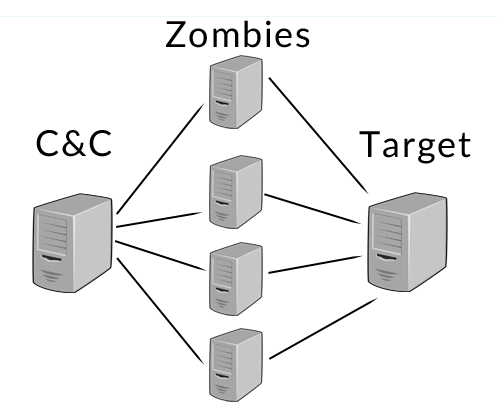
\includegraphics[width=0.5\textwidth]{assets/botnet_example.png}
  \captionof{figure}{An example of the C\&C commanding the zombies to attack \textit{Target.}}
  \label{fig:botnet_example}
\end{center}

\section{Motivation}
It's difficult to justify the motivation behind infecting thousands of computers to
unwillingly act as one's personal army. Aside from deriving enjoyment from chaos,
it seems as though these motivations generally fall into two categories.

\subsection{Political}
In 2007 a botnet targeted the essential electronic infrastructure of the Republic
of Estonia \cite{estonia}. The attack brought down major banks, newspapers, and
even telecom companies. The inciting incident occurred when the Estonian government
removed a bronze statue from a city center built by the Soviets to commemorate those who died fighting
the Nazis in World War II \cite{estonia}. This act upset some political activists, who quickly
gained control of a botnet and unleashed it on the country.  Estonia remained under
fire for exactly two weeks, after which the barrage of traffic abruptly stopped.
This incident was the first of its kind, and revealed the unreasonable effectiveness
of botnets being used for politically motivated attacks.

\subsection{Economic}
To get an idea of the relative ease involved in purchasing a botnet, a Google
search for \quotes{\textit{botnets for sale}} garners 158,000 results.
The first of which is a website titled \quotes{\textbf{Hack Forums - Botnets, IRC Bots, and Zombies}},
where one can purchase pre-built botnets under a variety of different pricing schemes.
Recently a botnet containing 100,000 zombies claiming to be able to produce
1 terabit of traffic per second (enough bandwidth to make a relatively powerful server sweat)
was seen for sale for \$7,500 USD\cite{forbessale}. The underground market willing
to pay big money for powerful botnets provides a monetary incentive for the creators to make
their software as intrusive as possible.  The more zombies a botnet has control
of, the higher the price it will fetch.

\section{Mechanics}

\subsection{The Life Cycle of a Botnet}
\subsubsection{Recruitment}
In order to be effective, a botnet must have a large collection of zombies within its network of control.
Botnet creators commonly use a type of malware called a \textbf{worm} to recruit new members
\cite{lifecycle}.
Worms can be distinguished from other forms of malware by their ability to self replicate
in order to spread to other computers on the same network \cite{virustypes}.
This property is attractive to botnet creators as it promotes rapid spreading of the virus across
multiple hosts, and each new zombie adds an additional degree of separation from the source.
The techniques used to infect the initial set of zombies are consistent with
those used in general virus spreading.  These techniques may include social engineering,
embedding the virus in email attachments, and disguising the worm in phoney adware.
Once a new zombie is infected it \quotes{phones home} to the C\&C to register
itself as a member of the botnet, and then lays dormant awaiting a command
\cite{topology}.

\subsubsection{Command Propagation}
Once a sizeable network of zombies is formed the C\&C needs a mechanism for
relaying commands and updates. Interestingly, many of the different network topologies
used to accomplish this bear similarities to those used in non-malicious settings.
The main topologies are classified as follows:

\paragraph{Star \cite{topology}}
A single C\&C point of contact performs all communication with the members
of the botnet. This type of topology can be observed in Local Area Networks
where all computers are connected to the internet through a single router. As a
result it typically does not scale well with an increased number of zombies.

\begin{center}
  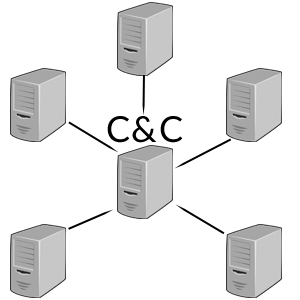
\includegraphics[width=0.5\textwidth]{assets/startopo.png}
  \captionof{figure}{A botnet with a star communication topology}
  \label{fig:star_topo_fig}
\end{center}

\begin{tabular}{p{8cm} | p{8cm}}
  \textbf{Pros} & \textbf{Cons} \\ \hline
  \textbullet{}Simple to implement                                    & \textbullet{}Single point of failure \\
  \textbullet{}Allows for rapid communication of commands and updates & \textbullet{}Large amount of network traffic traveling to and from single location\\
                                                                      & \textbullet{}Easier to locate C\&C
\end{tabular}

\paragraph{Multiserver \cite{topology}}
Multiple interconnected C\&C servers coordinate to distribute messages to the zombies.
Thoughtful geographical placement of these C\&C servers can reduce latency across
large distances.  This technique can be seen at the global network core where each
Internet Service Provider (ISP) provides internet connection to a small subset of the population, with support for
inter-ISP communication across long distances.

\begin{center}
  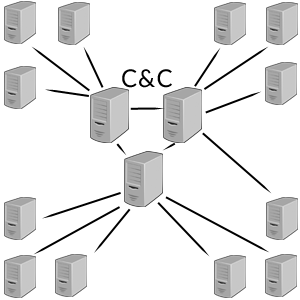
\includegraphics[width=0.5\textwidth]{assets/multiservertopo.png}
  \captionof{figure}{A botnet with a multiserver communication topology}
  \label{fig:mulitserver_topo_fig}
\end{center}

\begin{tabular}{p{8cm} | p{8cm}}
  \textbf{Pros} & \textbf{Cons} \\ \hline
  \textbullet{}Reduced load on each C\&C                    & \textbullet{}Difficult initial setup \\
  \textbullet{}Zombies can failover in case of a C\&C crash & \textbullet{}Complicated to coordinate\\
  \textbullet{}Optimized for long distance communication    & \\
\end{tabular}

\paragraph{Peer to Peer (P2P) \cite{topology}}
In a P2P botnet there is no centralized C\&C, commands can be injected via any zombie.
Each zombie that receives a command will then fan it out to all known peers.
Generally these commands are signed with some sort of secret key to verify they
are coming from an authoritative source \cite{topology}. P2P botnets generally
feature many redundant connections so that in the event one of the zombies is
shut down, commands can still reach the rest of the network \cite{topology}.
Dismantling a botnet organized in this manner has proved to be very difficult as
it requires that each individual member rids itself of the offending malware.
This type of network topology is most famously used in BitTorrent,
a service where peers can directly share files with one another without the need for a central
repository.

\begin{center}
  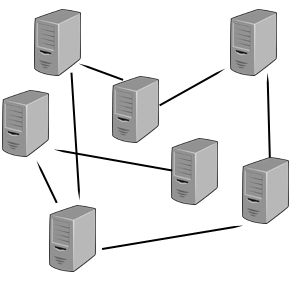
\includegraphics[width=0.5\textwidth]{assets/p2ptopo.png}
  \captionof{figure}{A botnet with a P2P communication topology.  Note the lack of explicit C\&C}
  \label{fig:p2p_topo_fig}
\end{center}

\begin{tabular}{p{8cm} | p{8cm}}
  \textbf{Pros} & \textbf{Cons} \\ \hline
  \textbullet{}No central point of contact  & \textbullet{}Command propagation may be slow \\
  \textbullet{}Difficult to shut down       & \textbullet{}Members can be discovered by observing fanout messages\\
                                            & \textbullet{}Infected users may notice spikes in bandwidth usage\\
\end{tabular}

\subsubsection{Attack}
Once a botnet has been constructed and a communication infrastructure has been put into
place, the bot master can issue commands to the zombies to carry out attacks.
As stated earlier, there are two main attack vectors utilized by botnets, as follows:

\paragraph{Distributed Denial of Service Attacks (DDos)}
DDoS attacks are among the least elegant of cyber attacks. Essentially, each
zombie in the botnet is ordered to repeatedly send requests to a given server.
The goal is to saturate this server with requests to the point where it
can no longer service legitimate users.  These types of attacks are particularly
difficult to handle as the server cannot simply ignore requests from a single host,
it must distinguish legitimate users from members of the botnet.
This is a non-trivial task and is further discussed in Section \ref{detection}.

\paragraph{Sending of Spam Emails}
Since sending thousands of emails from a single server/address is sure to raise a red flag
in spam detection softwares, botnets are used to distribute the load.  Each zombie
in the botnet is ordered to send a small subset of the desired emails. No single zombie
is generating enough emails to seem suspicious, but collectively a massive amount
of emails are being created. These emails typically contain paid-for advertisements
and malware riddled attachments.

\subsection{Techniques For Remaining Undetected}
Aside from infecting as many hosts as possible, the main goal for botnet owners
is to remain undetected by employing the following methods:

\subsubsection{Encrypted Communication Protocols}
To provide better security and help prevent other users from hijacking botnets,
C\&Cs can communicate with zombies (and vice versa) via encrypted protocols.
Increasingly botnets are moving to encrypted HTTP based protocols instead of
the once used plain text Internet Relay Chat (IRC) protocol \cite{botlab}.

\subsubsection{Polymorphic Packers}
Signature matching is a popular technique used in anti-virus software.  Once a new
virus is discovered, a unique signature is generated by sampling sections of the
binary content of the file. In order to stop anti-virus software from detecting
zombie software this way, botnet creators use \textbf{polymorphic packers} \cite{botlab}.
Polymorphic packers are able to construct two binary files which act identically, but will
produce completely different signatures. In order to leverage this property, each
time a zombie infects a new host it polymorphically repacks its binary file.  The result
is thousands of different signatures for the same zombie software, making it virtually
impossible for a signature based anti-virus to discern any kind of similarity.

\subsubsection{Fast Flux Domain Name System (DNS)}
Fast Flux is a technique which exploits the nature of DNS in order to hide illegal
operations inside of a botnet \cite{fastflux}. To fully understand how Fast Flux works,
some introductory knowledge on DNS is required.
\\ \\
\textbf{DNS} is a web protocol which, in a nutshell, provides name to address translation.
For example, when you attempt to visit \quotes{facebook.com}, your browser first makes a query to
a DNS server to resolve the name \quotes{facebook.com} to an internet address which can
be used to make a connection.  In this way \quotes{facebook.com} is simply a convenient
alias for some longer (and harder to memorize) address. It is possible, and actually
beneficial, that a single name may have multiple addresses associated with it. This phenomenon
allows DNS servers to provide a basic type of load balancing between multiple servers.
Finally, each DNS record (name to address pairing) also contains a field called
the \textbf{time to live (TTL)}. This field indicates that the given record is only
valid for some period of time, after which it should be invalidated and re-updated.
\\ \\
In order to take advantage of the dynamic nature of DNS records, botnet owners
quickly cycle the address mapped to the name of an illegal website with that
of members in the botnet \cite{fastflux}. These mappings are assigned an unusually low TTL
(between 1 and 15 minutes), after which the address will be re-mapped to a
different member of the botnet.  These members act as proxies, forwarding requests to other proxies,
eventually leading to the actual server hosting the illegal content,
dubbed the \textbf{mothership} \cite{fastflux}. Consequently the set of suspected
hosts is in constant flux, leaving only one option to disrupt the malicious network:
shutting down the offending domain name at the registrar level \cite{fastflux}.
Unfortunately many registrars are hesitant to deactivate Fast Flux domains as they
provide them with a steady stream of revenue \cite{fastflux}.


\section{Detecting Botnets Using Unsupervised Clustering}
\label{detection}

Unsupervised clustering is a common statistical analysis technique which partitions a set of unlabeled
observations into subsets known as \textbf{clusters}.  These clusters are formed in
such a way that observations within the
same cluster are more similar to each other, by some similarity metric, than
those in other clusters. A tool named BotMiner was developed in 2008 which examines
activity on large networks and performs clustering on the hosts \cite{clustering}.
The algorithm takes advantage of the fact that hosts belonging to a botnet will most
likely exhibit similar behaviour, and therefore fall into the same cluster.
To accomplish this, BotMiner uses two different similarity metrics: activity and
communication \cite{clustering}.  Activity clustering groups hosts based on the
types of activities they perform (e.g. port scanning, spamming, file downloading,
etc.) \cite{clustering}.  Activity clustering provides a high level model of which
hosts in the network have a tendency to perform similar tasks, but does not contribute enough
information to be conclusive.  To aid in developing a low level understanding
of the network, communication clustering is also performed \cite{clustering}.
Communication clustering determines similarity using attributes such as average
number of bytes sent per connection, average number of connections per hour, etc.
These two types of clusters are then intersected, resulting in the potential
botnets \cite{clustering}.  What makes this approach significant to the security community
is that it assumes nothing about the specific structure or communication protocols of
the botnets in question, but relies only on their general nature.

\section{Analysis of Historical Botnets}

\subsection{Conficker}
The Conficker worm was first seen in 2008 and has since infected an estimated
7-15 million hosts \cite{conficker}.  The worm targeted only Windows based machines,
and used a combination of dictionary password attacks, and a known NetBIOS
vulnerability to gain access \cite{conficker}.
Conficker utilized an advanced
polymorphic packer which shuffled its machine code sequence and then re-assembled
it using \textit{jmp} instructions.  This protected Conficker from signature
based anti-virus software.  Once Conficker gained control of a machine it killed
all anti-virus related
processes on the host and blocked multiple security websites, preventing users
from accessing removal tools \cite{conficker}.  In order to mask communication
with the C\&C, Conficker used a technique known as \textbf{Domain Flux}. Domain
Flux operates similarly to Fast Flux but instead of remapping the address of a
single domain to multiple hosts,
new domains are continually registered and mapped to the same host.
Newly infected zombies would
synchronize clocks with their infector, and this clock value would be used as a
seed to randomly generate multiple \quotes{Call Home} domains each day \cite{conficker}.
Only a portion of these domains would actually resolve to the C\&C, leaving security
researchers to probe the entire list in search of the culprit.  Conficker used an
encrypted P2P protocol to propagate updates and pass arbitrary binary files
through the network. These binary files could be used to carry out complicated
tasks not directly supported by the communication protocol \cite{conficker}.
Eventually Microsoft patched the vulnerabilities that Conficker used to spread,
and the \textit{Conficker Working Group} was formed with the goal of disrupting
the flux of \quotes{Call Home} domains generated each day.  These two efforts have
drastically slowed the spread of the virus.

\subsection{Stuxnet}
Stuxnet is a unique form of botnet, often regarded as the first cyber
warfare weapon ever \cite{stuxnet}. Stuxnet
was developed to specifically target \textbf{programmable logic controllers (PLCs)},
a category of computer used to control machinery such as assembly lines,
vending machines, and even nuclear centrifuges \cite{stuxnet}.  Ralph Langner,
the researcher who discovered Stuxnet, has speculated (but never proven)
that Stuxnet was created by the governments of the United States and Israel with the intent of
targeting high-value infrastructure in Iran. The worm spread mainly via USB drives,
closely monitoring the ports of its host and jumping to any USB device that was connected.
Stuxnet would then latch onto any Windows based machine it came in
contact with, but if the host was not running PLC software it remained mostly dormant.
If the worm found a PLC machine it would load malicious code onto the controller
with the intent of causing physical damage to the connected machinery. Stuxnet exploited the fact that most
PLCs did not perform any kind of validation on the instructions they received.
The addition of this class of safeguard relied on updates from the PLC manufacturers, who were
initially unresponsive \cite{stuxnet}.
The worm had very little interaction with the C\&C servers, checking in only
to provide a notification of infection \cite{stuxnet}.  If two Stuxnet instances
came in contact with one another they would compare version numbers, and
the newer worm would update the older one \cite{stuxnet}. Strangely, the source
code for Stuxnet included a time-based kill switch which instructed the malware
to cease spreading after June 24, 2012.

\subsection{Mirai}
A botnet constructed by the Mirai worm was responsible for the most recent massive internet
outage, affecting major websites such as Twitter, Facebook, Reddit, Github and Spotify.
The attack targeted \textit{Dyn DNS}, a large scale DNS provider
which boasts multiple big name clients \cite{mirai}.
Mirai was developed to take advantage of the surge in insecure internet connected
household devices, known as \textbf{Internet of Things (IoT) Devices}.
The majority of these IoT devices are produced by companies
who have very little experience in internet security, and thus lack
basic layers of protection.  The technique used by the Mirai worm to infect hosts is embarrassingly simple:
Scan the network looking for IoT devices, and then attempt to gain access by
cycling through 62 different username/password combinations \cite{mirai}.
Mirai's username/password dictionary is unusually small, but includes commonly
used default combinations among IoT device vendors.  For example, a Chinese company
named XiongMai Technologies uses \textit{root/xc3511} as default authentication credentials
for a large portion of their devices, a combination which appears in Mirai's dictionary.
In an official statement, Dyn DNS's Chief Strategy Officer stated 
\quotes{We observed 10s of millions of discrete IP addresses associated with the
Mirai botnet that were part of the attack.} \cite{dyndns}
This implies that 10s of millions of IoT devices were using only 62 distinct
username/password combinations. Most IoT devices do not provide an interface for
the owner to change the username or password, so currently the only solution is to
disconnect the compromised device or firewall incoming connections to popular
botnet ports (22, 23, 80). Soon after the massive attack, the source code for the
Mirai worm was released and is now being hosted on Github.com. This open sourcing
will likely be followed by more infected devices, as it provides an open forum
for malicious users to use and even improve the malware. IoT devices will
most likely remain insecure for some time until a set of strict regulations are
published, and security audits are performed on new devices to ensure they conform
to these regulations before they are released.

% Maybe drop this section?
%\section{Legal/Consenual Botnets}
%Research, lulz lazor, etc.

\section{Conclusion}
Botnets are still, and probably will be for some time, a legitimate internet threat.
The Mirai attack is evidence that even though many organizations are becoming more
security aware, zombies spread across the devices of a few negligent vendors can
wreak enough havoc to produce massive internet outages.
Given that the amount of disruption a botnet is able to cause is in direct
correlation with the network speed of its members, the recent advent of ultra fast fiber
optic internet connection will only increase their effectiveness. Protocol
independent detection systems, as mentioned in Section \ref{detection},
will be a crucial mitigation asset, as they are immune to the constantly changing 
malware landscape.  Ultimately security regulations and mandatory audits
for companies producing internet connected devices will be necessary to truly
suppress the threat that botnets pose. 

\pagebreak
\begin{thebibliography}{1}
  \bibitem{kapersky} Kapersky Lab. {\em What is a Botnet Attack?}
    usa.kaspersky.com.

  \bibitem{lifecycle} R. A. Rodriguez-Gomez, G. Maciá-Fernández. {\em Analysis of botnets through life-cycle} 2011:
  Proceedings of the International Conference on Security and Cryptography.

  \bibitem{virustypes} Cisco. {\em What Is the Difference: Viruses, Worms, Trojans, and Bots}
    cisco.com.

  \bibitem{malwareprop} MR. Faghani, H. Saidi. {\em Malware Propagation in Online Social Networks} 2009:
  Proceedings of the 4th IEEE International Conference on Malicious and Unwanted Software.

  \bibitem{topology} G. Ollmann. {\em Botnet Communication Topologies} 2009:
    www.damballa.com.

  \bibitem{forbessale} T. Fox-Brewster. {\em Hackers Sell \$7,500 IoT Cannon To Bring Down The Web Again} 2016:
    forbes.com.

  \bibitem{estonia} J. Davis. {\em Hackers Take Down the Most Wired Country in Europe} 2007:
    wired.com.

  \bibitem{fbi} J. Demarest. {\em Taking Down Botnets} 2014:
    Statement Before the Senate Judiciary Committee, Subcommittee on Crime and Terrorism.

  \bibitem{botlab} JP. John. {\em Studying Spamming Botnets Using Botlab}  2009:
    USENIX Symposium on Networked Systems Design and Implementation (NSDI).

  \bibitem{fastflux} J. Nazario. {\em As the net churns: Fast-flux botnet observations}  2008:
     Malicious and Unwanted Software, 2008. MALWARE 2008. 3rd International Conference.

  \bibitem{clustering} G. Gu. {\em BotMiner: Clustering Analysis of Network Traffic for Protocol-and Structure-Independent Botnet Detection}  2008:
     USENIX Security Symposium, 2008.

  \bibitem{conficker} S. Shin. {\em Conficker and beyond: a large-scale empirical study}  2010:
    Proceedings of the 26th Annual Computer Security Applications Conference.

  \bibitem{stuxnet} R. Langner. {\em Stuxnet: Dissecting a cyberwarfare weapon}  2011:
     IEEE Security \& Privacy.

  \bibitem{mirai} I. Zeifman. {\em Breaking Down Mirai: An IoT DDoS Botnet Analysis}  2016:
     incapsula.com.

  \bibitem{dyndns} K. York. {\em Dyn Statement on 10/21/2016 DDoS Attack}  2016:
     dyn.com.
\end{thebibliography}

\end{document}
